Als erstes wollen wir uns mit der Fourier-Analyse von Signalen besch"aftigen.
Hierbei ist das Ziel das Verhalten eines Signals im Frequenzbereich zu charakterisieren.
Wir wollen jedoch in unserer Analyse davon ausgehen, dass wir ein Signal $x[\cdot]$ vorliegen haben, dessen spektrale Eigenschaften \emph{zeitvariant} sind.
Hiermit ist \emph{nicht} gemeint, dass wir davon ausgehen, dass das Signal zeitvariant ist, denn das ist es nat"urlich.
Es geht darum, dass der Anteil der verschiedenen Frequenzen in einem Signal sich mit der Zeit "andert.
Nat"urlich ist hier eine der am einfachsten zug"anglichen Anwendungen die Analyse von Audiosignalen.

\begin{listing}[ht]
    \noindent
    \begin{minipage}{0.51\textwidth}
        \strut\vspace*{-\baselineskip}\newline
        \inputminted[firstline=10, lastline=44]{python3}{code/stft_1.py}
    \end{minipage}%
    \begin{minipage}{0.48\textwidth}
        \strut\vspace*{-\baselineskip}\newline
        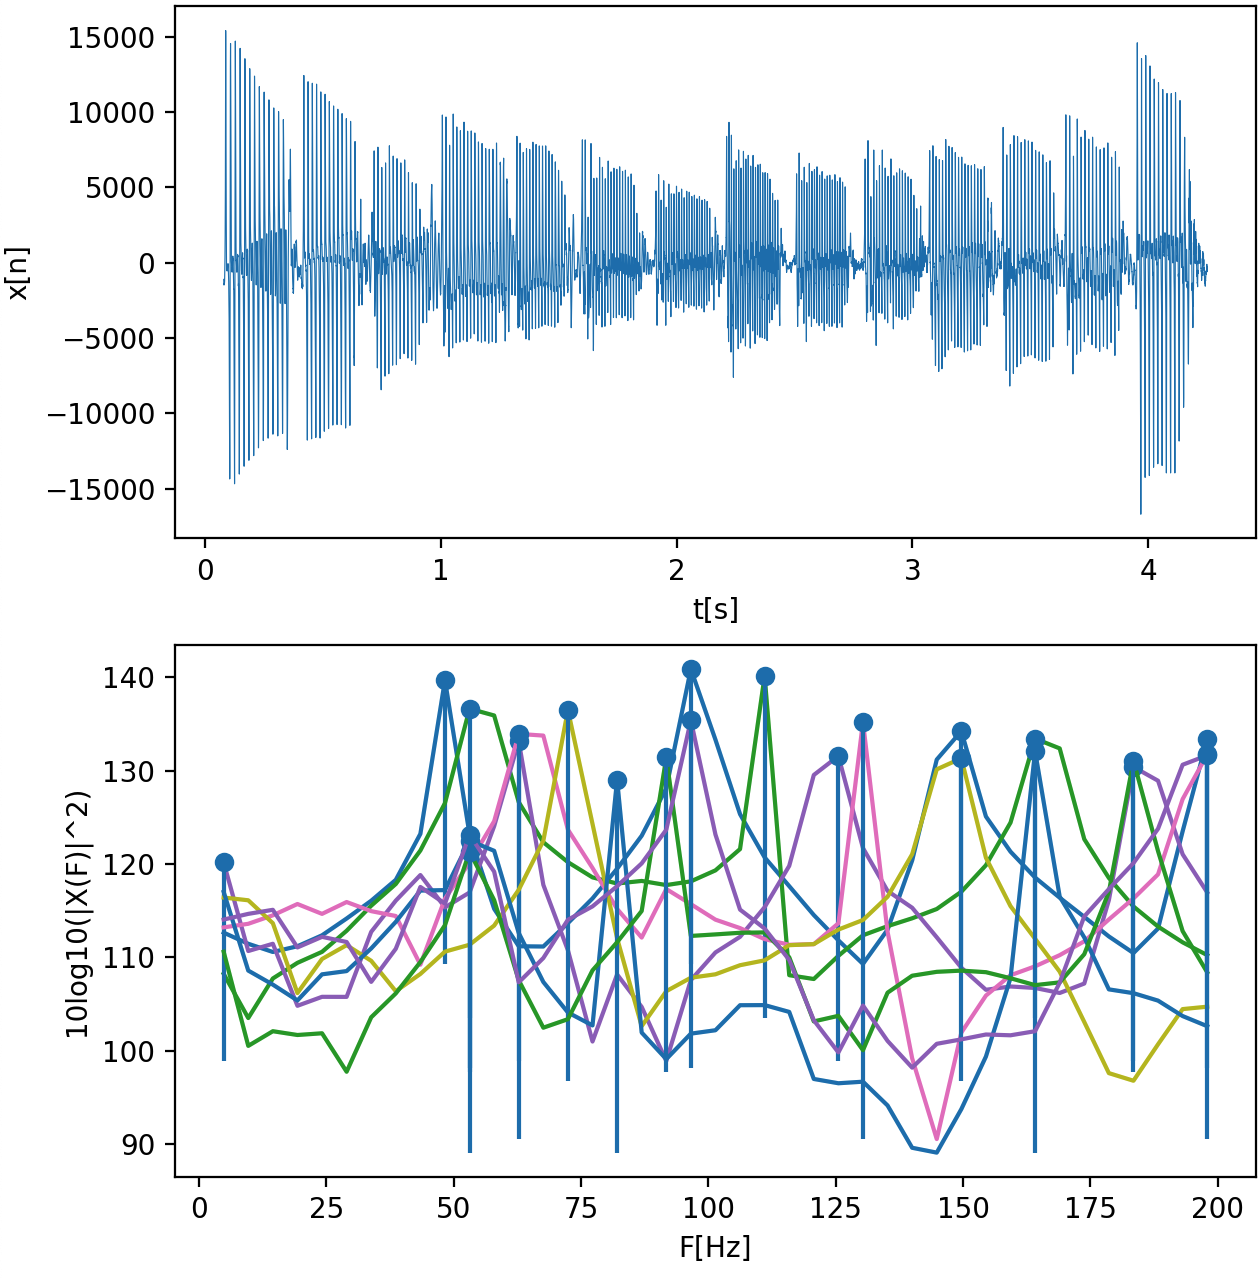
\includegraphics[width=\textwidth]{code/stft_1.png}

\begin{minted}{python}
[ 48.2811  96.5622 149.6715 197.9527]
[ 53.109  111.0466 164.1559]
[  4.8281  62.7654 125.5309 183.4683]
[ 62.7654 130.3590 197.9527]
[ 72.4217 149.6715]
[ 53.109   82.0779 164.1559]
[ 53.109   91.7341 183.4683]
[ 53.109   96.5622 197.95270418]
\end{minted}
    \end{minipage}
    \codecaption{dsv/code/stft_1.py}{Analyse einer \q{Bassline}, die eine G-Dur-Tonleiter spielt.}\label{py:stft_1}
\end{listing}

